\Object{Sémaphore a compte}
{
Le sémaphore a compte est un objet permettant de protéger une ressource
critique. On peut représenter le sémaphore par analogie avec une boite qui
contient un certain nombre de jetons. Des utilisateurs se partageant une
ressource ne peuvent y accéder qu'à la condition de \emph{prendre} un jeton
disponible, et le \emph{rendent} une fois qu'ils n'ont plus besoin de la
ressource critique.
}
{
\begin{itemize}
	\item Capacité (nombre de jetons qu'il peut contenir) \lstinline{int}
	\item Etat (nombre de jetons qu'il contient à un instant t) \lstinline{int}
\end{itemize}

Le sémaphore est représenté et manipulé par l'utilisateur grâce à un
identifiant communiqué à l'utilisateur lors de l'initialisation de l'objet
(symbole de type \texttt{semid\_t}).
}
{
\begin{itemize}
	\item \lstinline{semid\_t creerSemaphore(int maxJetons, int initJetons)}
L'initialisation d'un sémaphore permet de créer l'objet. L'utilisateur définit
le nombre de jetons qu'il peut contenir et le nombre qu'il contient à la
création de l'objet. \texttt{maxJeton} correspond au maximum de jetons que peux
accueillir le sémaphore et \texttt{initJetons} le nombre de jeton initial.
	\item \lstinline{void supprSemaphore(semid\_t semId)} La déstruction d'un
sémaphore détruit l'objet et le supprime de la mémoire. Si des utilisateurs
attendaient la libération d'un jeton, alors ils seront libérés et l'utilisateur
sera notifié par un code retour particulier (voir ci-dessous).
	\item \lstinline{int prendre(semid\_t semId, int attendre)} L'utilisateur
souhaitant accéder à la ressource partagée doit prendre un jeton dans le
sémaphore. Il peut spécifier la stratégie d'attente si aucun jeton n'est
disponible. La fonction retourne 1 si l'utilisateur a obtenu un jeton, 0 si non
et -1 si le sémaphore identifié par semId n'existe pas. le paramètre
\texttt{attendre} vaut 0 si l'utilisateur ne souhaite pas attendre, -1 pour
attendre indéfiniment ou tout autre valeur correspondant à la durée d'attente
en millisecondes.
	\item \lstinline{int donner(semid\_t semId)} L'utilisateur souhaite
déposer un jeton dans le sémaphore. Les codes retour de la fonction sont les
suivants : 1 si le jeton a été rendu, 0 si le sémaphore est plein, -1 si le
sémaphore identifié par semId n'existe pas. Ce mécanisme ne vérifie pas si un
utilisateur a pris un jeton avec \texttt{prendre()} avant de le donner avec
\texttt{donner()}.
\end{itemize}
}
{
\begin{figure} [htp]
\centering
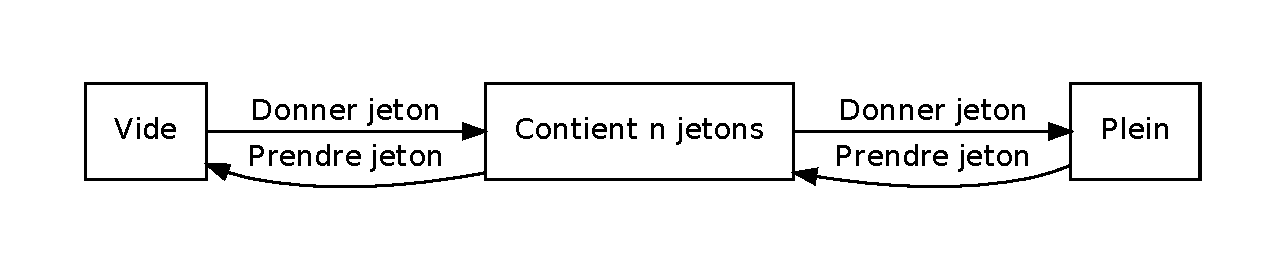
\includegraphics[width=\textwidth]{img/etatSemaphoreACompte.pdf}
\end{figure}
}
{
}
